\begin{table}[H]
\centering
\footnotesize
\definecolor{tabglobalgeneralunnorm0}{rgb}{0.854,0.0772,0.1193}
\definecolor{tabglobalgeneralunnorm1}{rgb}{0.7792,0.026,0.139}
\definecolor{tabglobalgeneralunnorm2}{rgb}{0.7979,0.0388,0.1341}
\definecolor{tabglobalgeneralunnorm3}{rgb}{0.8446,0.0708,0.1218}
\definecolor{tabglobalgeneralunnorm4}{rgb}{0.6896,0.0,0.149}
\definecolor{tabglobalgeneralunnorm5}{rgb}{0.7346,0.0,0.149}
\definecolor{tabglobalgeneralunnorm6}{rgb}{0.8212,0.0548,0.128}
\definecolor{tabglobalgeneralunnorm7}{rgb}{0.517,0.0,0.149}
\definecolor{tabglobalgeneralunnorm8}{rgb}{0.592,0.0,0.149}
\definecolor{tabglobalgeneralunnorm9}{rgb}{0.502,0.0,0.149}
\definecolor{tabglobalgeneralunnorm10}{rgb}{0.6145,0.0,0.149}
\definecolor{tabglobalgeneralunnorm11}{rgb}{0.7932,0.0356,0.1353}
\definecolor{tabglobalgeneralunnorm12}{rgb}{0.6971,0.0,0.149}
\definecolor{tabglobalgeneralunnorm13}{rgb}{0.8025,0.042,0.1329}
\definecolor{tabglobalgeneralunnorm14}{rgb}{0.7838,0.0292,0.1378}
\definecolor{tabglobalgeneralunnorm15}{rgb}{1.0,0.9801,0.7513}
\definecolor{tabglobalgeneralunnorm16}{rgb}{1.0,0.9402,0.6538}
\definecolor{tabglobalgeneralunnorm17}{rgb}{0.9984,0.8971,0.5596}
\definecolor{tabglobalgeneralunnorm18}{rgb}{0.9961,0.8498,0.4615}
\definecolor{tabglobalgeneralunnorm19}{rgb}{0.9961,0.7634,0.3684}
\definecolor{tabglobalgeneralunnorm20}{rgb}{0.9955,0.6781,0.2894}
\definecolor{tabglobalgeneralunnorm21}{rgb}{0.9933,0.5962,0.254}
\definecolor{tabglobalgeneralunnorm22}{rgb}{0.991,0.4793,0.2143}
\definecolor{tabglobalgeneralunnorm23}{rgb}{0.9888,0.3398,0.1744}
\definecolor{tabglobalgeneralunnorm24}{rgb}{0.9463,0.2187,0.1412}
\definecolor{tabglobalgeneralunnorm25}{rgb}{0.8867,0.0996,0.1107}
\definecolor{tabglobalgeneralunnorm26}{rgb}{0.7046,0.0,0.149}
\definecolor{tabglobalgeneralunnorm27}{rgb}{0.5695,0.0,0.149}
\definecolor{tabglobalgeneralunnorm28}{rgb}{1.0,0.9934,0.7838}
\definecolor{tabglobalgeneralunnorm29}{rgb}{0.9863,0.3019,0.1636}
\definecolor{tabglobalgeneralunnorm30}{rgb}{0.9371,0.1995,0.1361}
\definecolor{tabglobalgeneralunnorm31}{rgb}{1.0,0.9911,0.7783}
\definecolor{tabglobalgeneralunnorm32}{rgb}{0.9094,0.1419,0.1206}
\definecolor{tabglobalgeneralunnorm33}{rgb}{0.9156,0.1547,0.124}
\definecolor{tabglobalgeneralunnorm34}{rgb}{1.0,0.9823,0.7567}
\definecolor{tabglobalgeneralunnorm35}{rgb}{0.9125,0.1483,0.1223}
\definecolor{tabglobalgeneralunnorm36}{rgb}{0.9525,0.2315,0.1447}
\definecolor{tabglobalgeneralunnorm37}{rgb}{1.0,0.9734,0.735}
\definecolor{tabglobalgeneralunnorm38}{rgb}{0.891,0.1036,0.1102}
\definecolor{tabglobalgeneralunnorm39}{rgb}{0.9899,0.4096,0.1943}
\definecolor{tabglobalgeneralunnorm40}{rgb}{1.0,0.9513,0.6809}
\definecolor{tabglobalgeneralunnorm41}{rgb}{0.7745,0.0228,0.1403}
\definecolor{tabglobalgeneralunnorm42}{rgb}{0.9923,0.5598,0.2382}
\definecolor{tabglobalgeneralunnorm43}{rgb}{1.0,0.9424,0.6593}
\definecolor{tabglobalgeneralunnorm44}{rgb}{0.622,0.0,0.149}
\definecolor{tabglobalgeneralunnorm45}{rgb}{0.9932,0.5916,0.252}
\definecolor{tabglobalgeneralunnorm46}{rgb}{1.0,0.938,0.6484}
\definecolor{tabglobalgeneralunnorm47}{rgb}{0.9936,0.6053,0.2579}
\begin{minipage}{0.34\textwidth}
\centering
\footnotesize vs.\ topological\\[3pt]
\renewcommand{\arraystretch}{1.2}
\begin{tabular}{lccc}
\toprule
Checkpoint & First & Middle & Last \\
\midrule
0 & \cellcolor{tabglobalgeneralunnorm0}\textcolor{white}{$0.437 \pm 0.041$} & \cellcolor{tabglobalgeneralunnorm1}\textcolor{white}{$0.472 \pm 0.047$} & \cellcolor{tabglobalgeneralunnorm2}\textcolor{white}{$0.463 \pm 0.040$} \\
1 & \cellcolor{tabglobalgeneralunnorm3}\textcolor{white}{$0.442 \pm 0.042$} & \cellcolor{tabglobalgeneralunnorm4}\textcolor{white}{$0.505 \pm 0.047$} & \cellcolor{tabglobalgeneralunnorm5}\textcolor{white}{$0.491 \pm 0.045$} \\
5 & \cellcolor{tabglobalgeneralunnorm6}\textcolor{white}{$0.453 \pm 0.040$} & \cellcolor{tabglobalgeneralunnorm7}\textcolor{white}{$0.554 \pm 0.051$} & \cellcolor{tabglobalgeneralunnorm8}\textcolor{white}{$0.534 \pm 0.045$} \\
15 & \cellcolor{tabglobalgeneralunnorm1}\textcolor{white}{$0.473 \pm 0.040$} & \cellcolor{tabglobalgeneralunnorm9}\textcolor{white}{$0.560 \pm 0.037$} & \cellcolor{tabglobalgeneralunnorm10}\textcolor{white}{$0.526 \pm 0.037$} \\
50 & \cellcolor{tabglobalgeneralunnorm11}\textcolor{white}{$0.464 \pm 0.038$} & \cellcolor{tabglobalgeneralunnorm8}\textcolor{white}{$0.532 \pm 0.048$} & \cellcolor{tabglobalgeneralunnorm12}\textcolor{white}{$0.502 \pm 0.040$} \\
200 & \cellcolor{tabglobalgeneralunnorm13}\textcolor{white}{$0.460 \pm 0.039$} & \cellcolor{tabglobalgeneralunnorm4}\textcolor{white}{$0.506 \pm 0.047$} & \cellcolor{tabglobalgeneralunnorm14}\textcolor{white}{$0.469 \pm 0.032$} \\
last & \cellcolor{tabglobalgeneralunnorm13}\textcolor{white}{$0.460 \pm 0.039$} & \cellcolor{tabglobalgeneralunnorm4}\textcolor{white}{$0.505 \pm 0.047$} & \cellcolor{tabglobalgeneralunnorm14}\textcolor{white}{$0.469 \pm 0.030$} \\
\bottomrule
\end{tabular}
\end{minipage}%
\hfill
\begin{minipage}{0.085\textwidth}
\centering
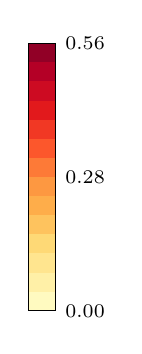
\begin{tikzpicture}
\fill[tabglobalgeneralunnorm15] (0,0.0000) rectangle (0.35,0.2429);
\fill[tabglobalgeneralunnorm16] (0,0.2429) rectangle (0.35,0.4857);
\fill[tabglobalgeneralunnorm17] (0,0.4857) rectangle (0.35,0.7286);
\fill[tabglobalgeneralunnorm18] (0,0.7286) rectangle (0.35,0.9714);
\fill[tabglobalgeneralunnorm19] (0,0.9714) rectangle (0.35,1.2143);
\fill[tabglobalgeneralunnorm20] (0,1.2143) rectangle (0.35,1.4571);
\fill[tabglobalgeneralunnorm21] (0,1.4571) rectangle (0.35,1.7000);
\fill[tabglobalgeneralunnorm22] (0,1.7000) rectangle (0.35,1.9429);
\fill[tabglobalgeneralunnorm23] (0,1.9429) rectangle (0.35,2.1857);
\fill[tabglobalgeneralunnorm24] (0,2.1857) rectangle (0.35,2.4286);
\fill[tabglobalgeneralunnorm25] (0,2.4286) rectangle (0.35,2.6714);
\fill[tabglobalgeneralunnorm13] (0,2.6714) rectangle (0.35,2.9143);
\fill[tabglobalgeneralunnorm26] (0,2.9143) rectangle (0.35,3.1571);
\fill[tabglobalgeneralunnorm27] (0,3.1571) rectangle (0.35,3.4000);
\draw[black,line width=0.3pt] (0,0) rectangle (0.35,3.4000);
\node[right,font=\scriptsize,anchor=west] at (0.35,3.4000) {0.56};
\node[right,font=\scriptsize,anchor=west] at (0.35,1.7000) {0.28};
\node[right,font=\scriptsize,anchor=west] at (0.35,0) {0.00};
\end{tikzpicture}
\end{minipage}%
\hfill
\begin{minipage}{0.34\textwidth}
\centering
\footnotesize vs.\ zero\\[3pt]
\renewcommand{\arraystretch}{1.2}
\begin{tabular}{lccc}
\toprule
Checkpoint & First & Middle & Last \\
\midrule
0 & \cellcolor{tabglobalgeneralunnorm28}\textcolor{black}{$0.172 \pm 0.143$} & \cellcolor{tabglobalgeneralunnorm29}\textcolor{white}{$7.619 \pm 6.955$} & \cellcolor{tabglobalgeneralunnorm30}\textcolor{white}{$8.361 \pm 7.008$} \\
1 & \cellcolor{tabglobalgeneralunnorm31}\textcolor{black}{$0.229 \pm 0.180$} & \cellcolor{tabglobalgeneralunnorm32}\textcolor{white}{$8.775 \pm 7.724$} & \cellcolor{tabglobalgeneralunnorm33}\textcolor{white}{$8.671 \pm 6.717$} \\
5 & \cellcolor{tabglobalgeneralunnorm34}\textcolor{black}{$0.399 \pm 0.287$} & \cellcolor{tabglobalgeneralunnorm35}\textcolor{white}{$8.718 \pm 7.220$} & \cellcolor{tabglobalgeneralunnorm36}\textcolor{white}{$8.101 \pm 6.057$} \\
15 & \cellcolor{tabglobalgeneralunnorm37}\textcolor{black}{$0.603 \pm 0.409$} & \cellcolor{tabglobalgeneralunnorm38}\textcolor{white}{$9.075 \pm 6.932$} & \cellcolor{tabglobalgeneralunnorm39}\textcolor{black}{$6.955 \pm 4.448$} \\
50 & \cellcolor{tabglobalgeneralunnorm40}\textcolor{black}{$1.064 \pm 0.573$} & \cellcolor{tabglobalgeneralunnorm41}\textcolor{white}{$10.240 \pm 6.554$} & \cellcolor{tabglobalgeneralunnorm42}\textcolor{black}{$6.004 \pm 3.448$} \\
200 & \cellcolor{tabglobalgeneralunnorm43}\textcolor{black}{$1.277 \pm 0.530$} & \cellcolor{tabglobalgeneralunnorm44}\textcolor{white}{$11.338 \pm 6.261$} & \cellcolor{tabglobalgeneralunnorm45}\textcolor{black}{$5.680 \pm 2.724$} \\
last & \cellcolor{tabglobalgeneralunnorm46}\textcolor{black}{$1.347 \pm 0.591$} & \cellcolor{tabglobalgeneralunnorm9}\textcolor{white}{$12.125 \pm 7.013$} & \cellcolor{tabglobalgeneralunnorm47}\textcolor{black}{$5.536 \pm 2.636$} \\
\bottomrule
\end{tabular}
\end{minipage}%
\hfill
\begin{minipage}{0.085\textwidth}
\centering
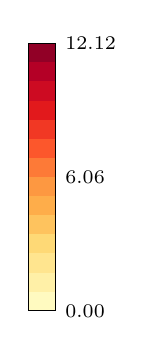
\begin{tikzpicture}
\fill[tabglobalgeneralunnorm15] (0,0.0000) rectangle (0.35,0.2429);
\fill[tabglobalgeneralunnorm16] (0,0.2429) rectangle (0.35,0.4857);
\fill[tabglobalgeneralunnorm17] (0,0.4857) rectangle (0.35,0.7286);
\fill[tabglobalgeneralunnorm18] (0,0.7286) rectangle (0.35,0.9714);
\fill[tabglobalgeneralunnorm19] (0,0.9714) rectangle (0.35,1.2143);
\fill[tabglobalgeneralunnorm20] (0,1.2143) rectangle (0.35,1.4571);
\fill[tabglobalgeneralunnorm21] (0,1.4571) rectangle (0.35,1.7000);
\fill[tabglobalgeneralunnorm22] (0,1.7000) rectangle (0.35,1.9429);
\fill[tabglobalgeneralunnorm23] (0,1.9429) rectangle (0.35,2.1857);
\fill[tabglobalgeneralunnorm24] (0,2.1857) rectangle (0.35,2.4286);
\fill[tabglobalgeneralunnorm25] (0,2.4286) rectangle (0.35,2.6714);
\fill[tabglobalgeneralunnorm13] (0,2.6714) rectangle (0.35,2.9143);
\fill[tabglobalgeneralunnorm26] (0,2.9143) rectangle (0.35,3.1571);
\fill[tabglobalgeneralunnorm27] (0,3.1571) rectangle (0.35,3.4000);
\draw[black,line width=0.3pt] (0,0) rectangle (0.35,3.4000);
\node[right,font=\scriptsize,anchor=west] at (0.35,3.4000) {12.12};
\node[right,font=\scriptsize,anchor=west] at (0.35,1.7000) {6.06};
\node[right,font=\scriptsize,anchor=west] at (0.35,0) {0.00};
\end{tikzpicture}
\end{minipage}
\caption{Global Wasserstein alignment, GeneralSheaf, unnormalised Laplacian. Mean $\pm$ SE across 10 datasets (First/Last), 8 for Middle (datasets with $L=2$ contribute no middle layer). Cell shading (each block independently scaled): white = 0, dark red = block maximum, YlOrRd colormap.}
\label{tab:global_general_unnorm}
\end{table}
